\chapter{Dependencies of \Routin}
In addition to the results for the low-mass region already shown in Section~\ref{sec:ROutIn}, the dependency of \Routin on \MET and \njets is also studied for the high-mass region. The corresponding results are shown in Figure~\ref{fig:ROutInDependencies2}. As for the low-mass region, no significant dependencies are observed.
\label{app:routin}

\begin{figure}[htbp]
\centering
\begin{minipage}[t]{0.49\textwidth}
  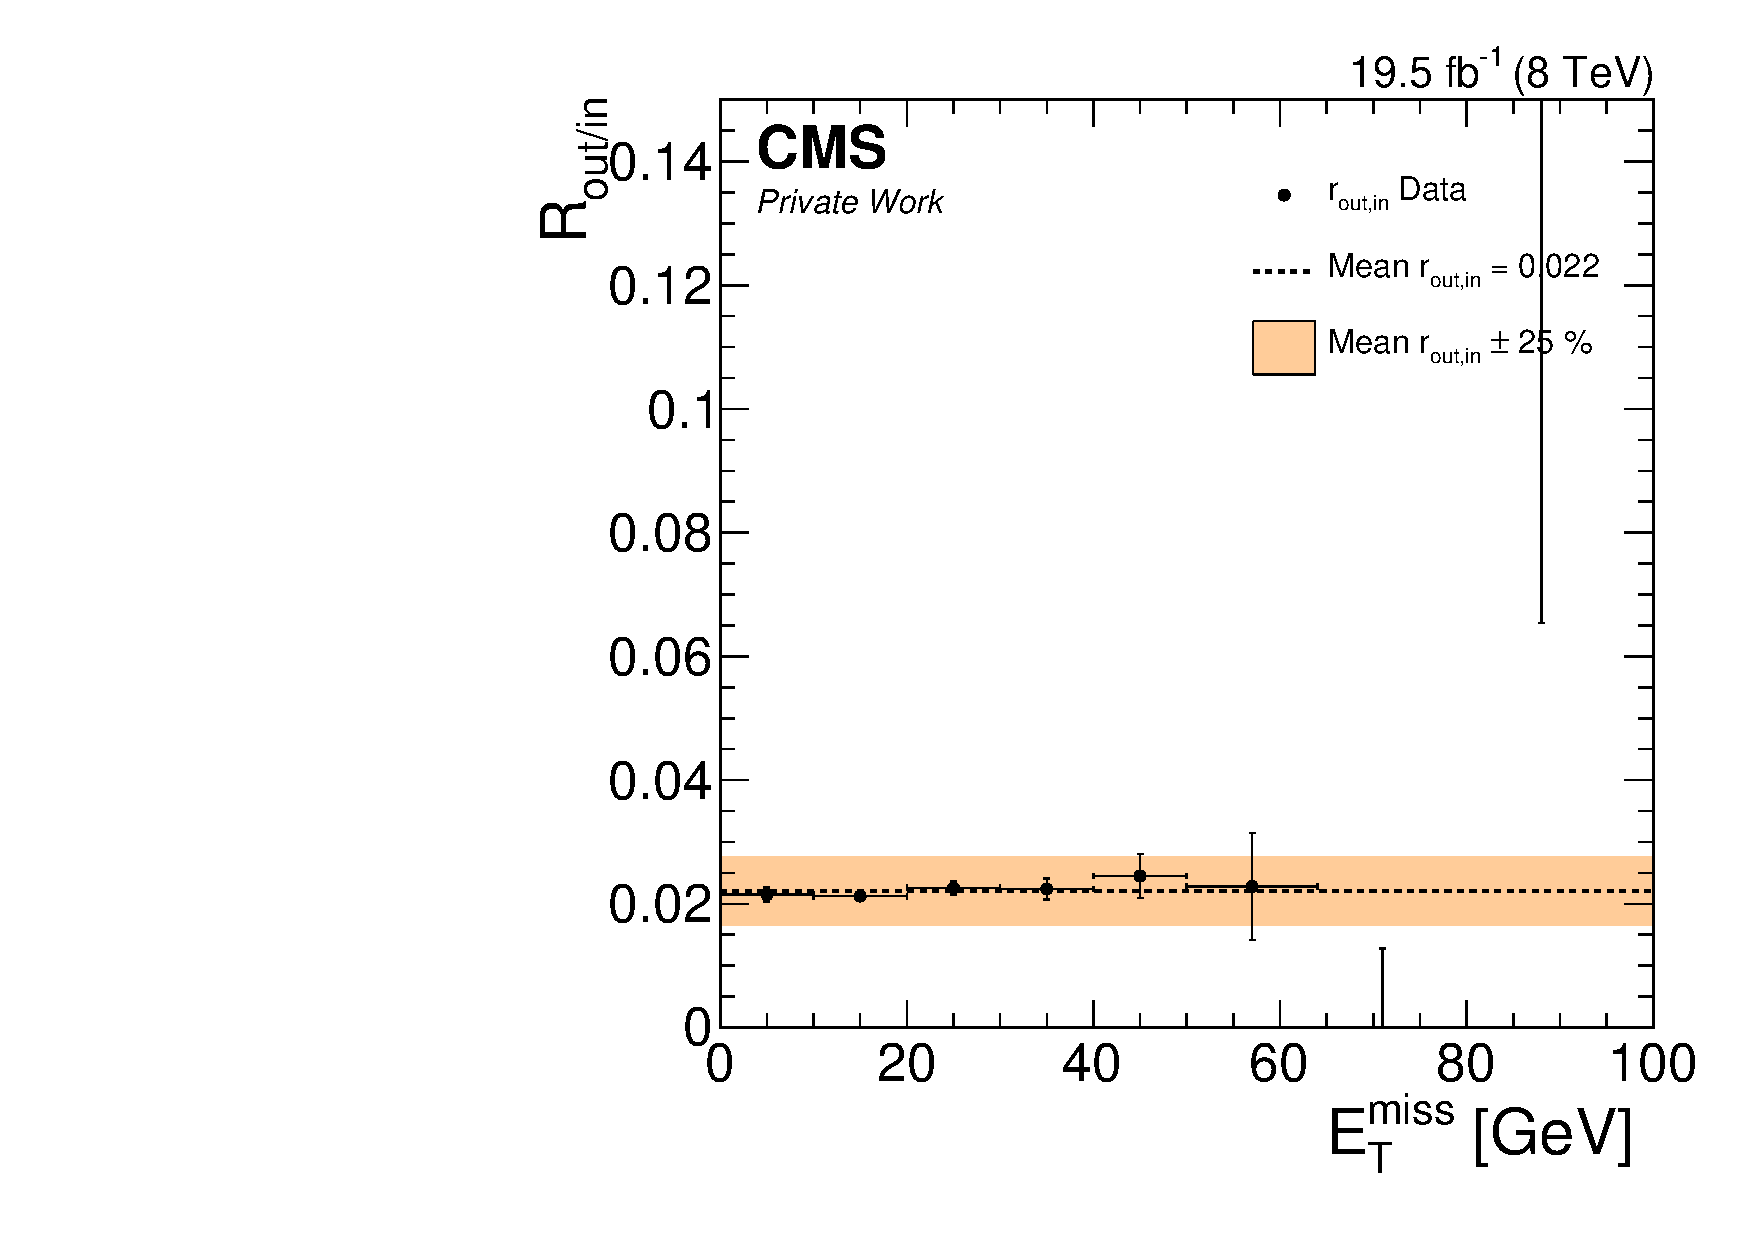
\includegraphics[width=\textwidth]{plots/BG/rOutIn/rOutInSyst_DrellYanControlCentral_Full2012_MET_HighMass_SF_None.pdf}
\end{minipage}
\begin{minipage}[t]{0.49\textwidth}
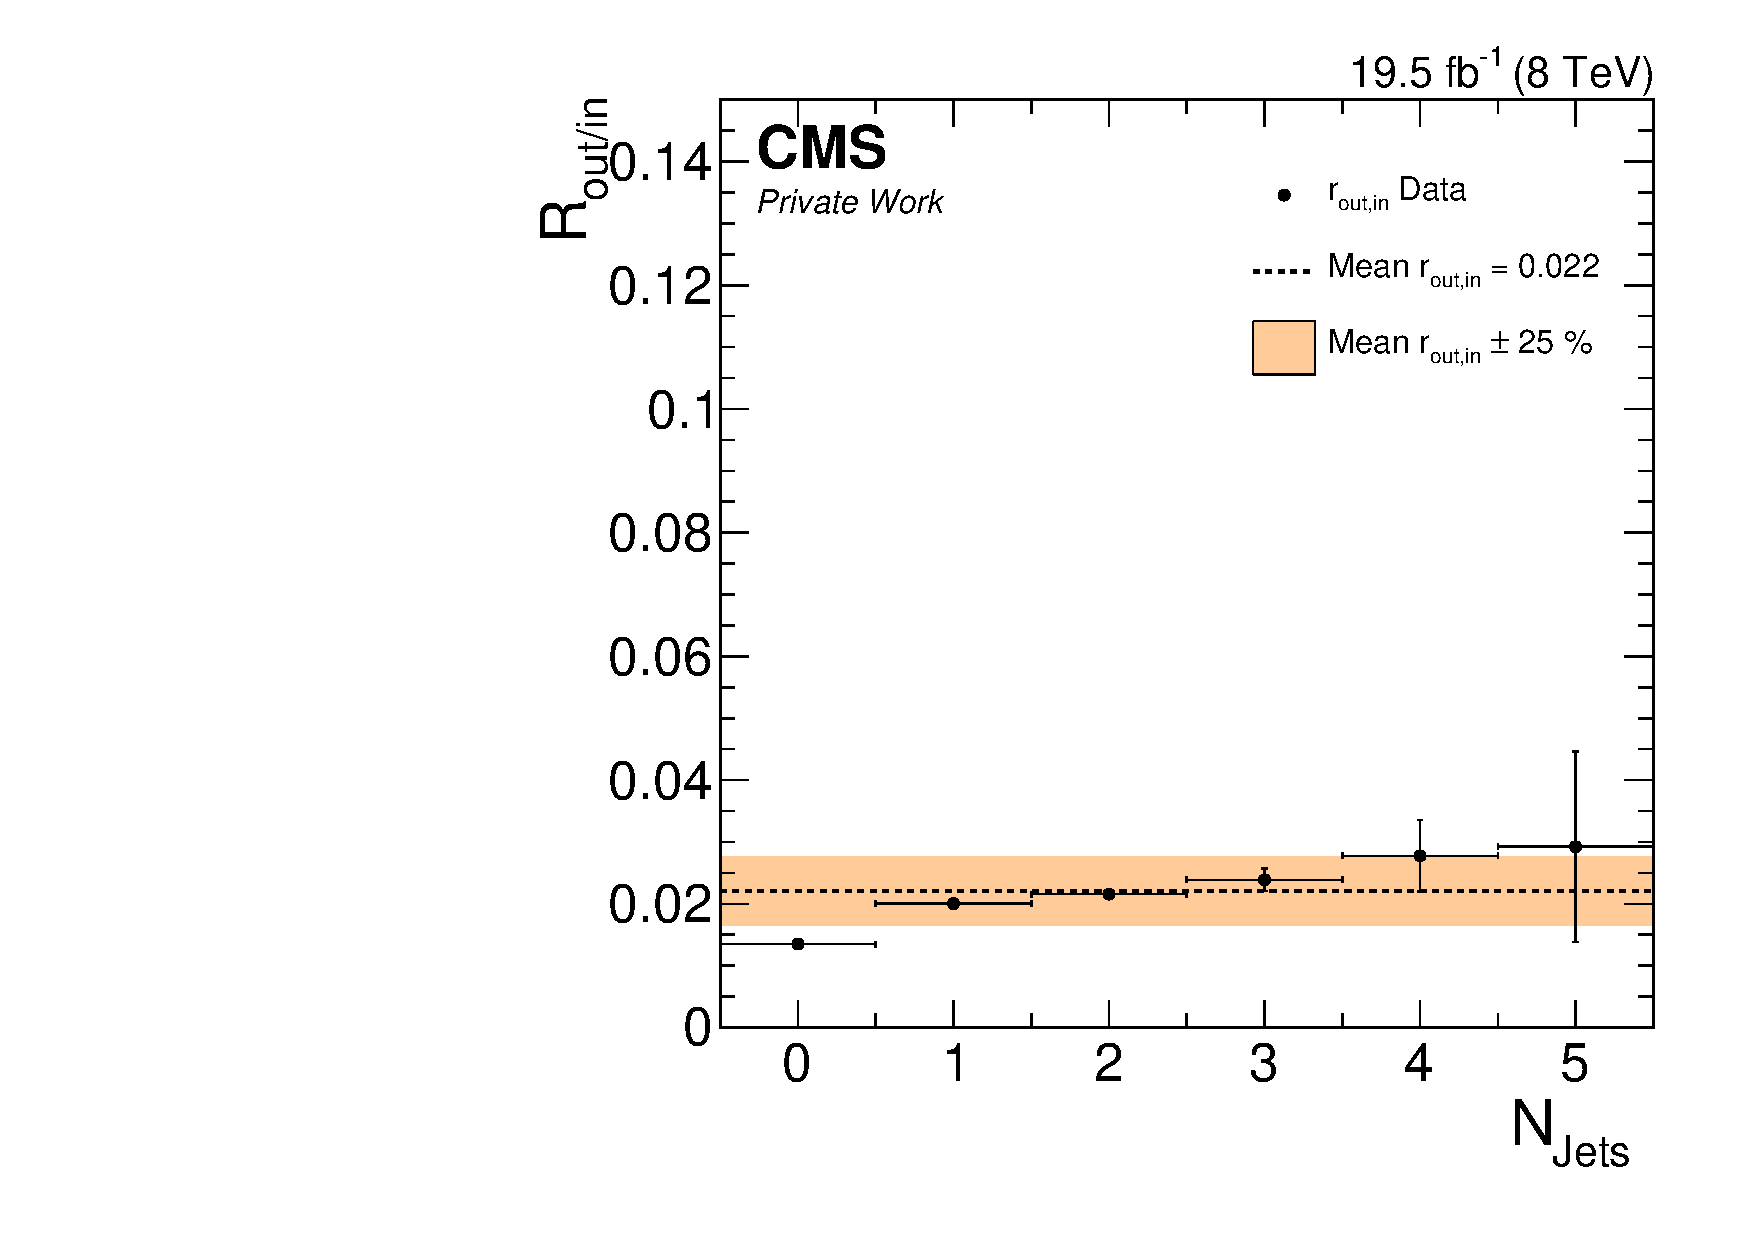
\includegraphics[width=\textwidth]{plots/BG/rOutIn/rOutInSyst_DrellYanControlCentral_Full2012_NJets_HighMass_SF_None.pdf}
\end{minipage}
\begin{minipage}[t]{0.49\textwidth}
  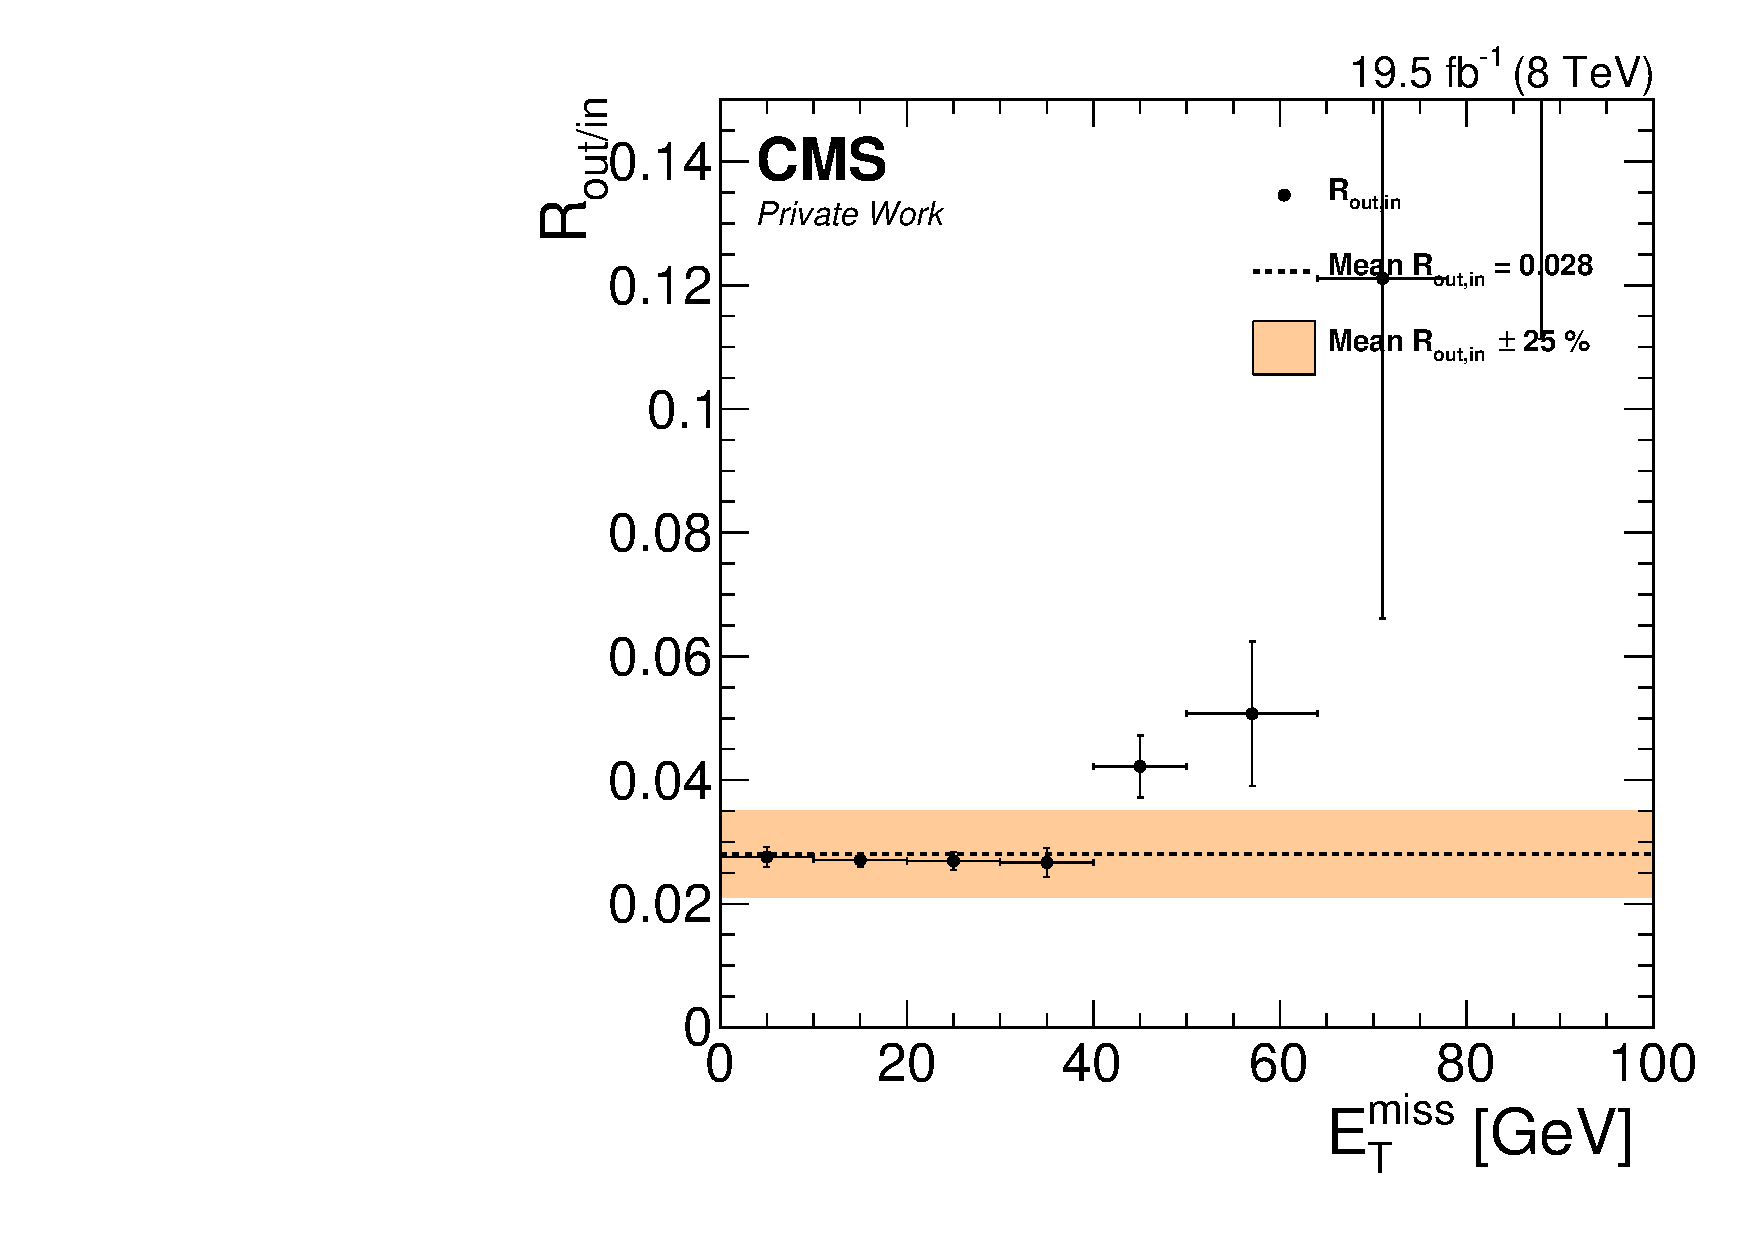
\includegraphics[width=\textwidth]{plots/BG/rOutIn/rOutInSyst_DrellYanControlForward_Full2012_MET_HighMass_SF_None.pdf}
\end{minipage}
\begin{minipage}[t]{0.49\textwidth}
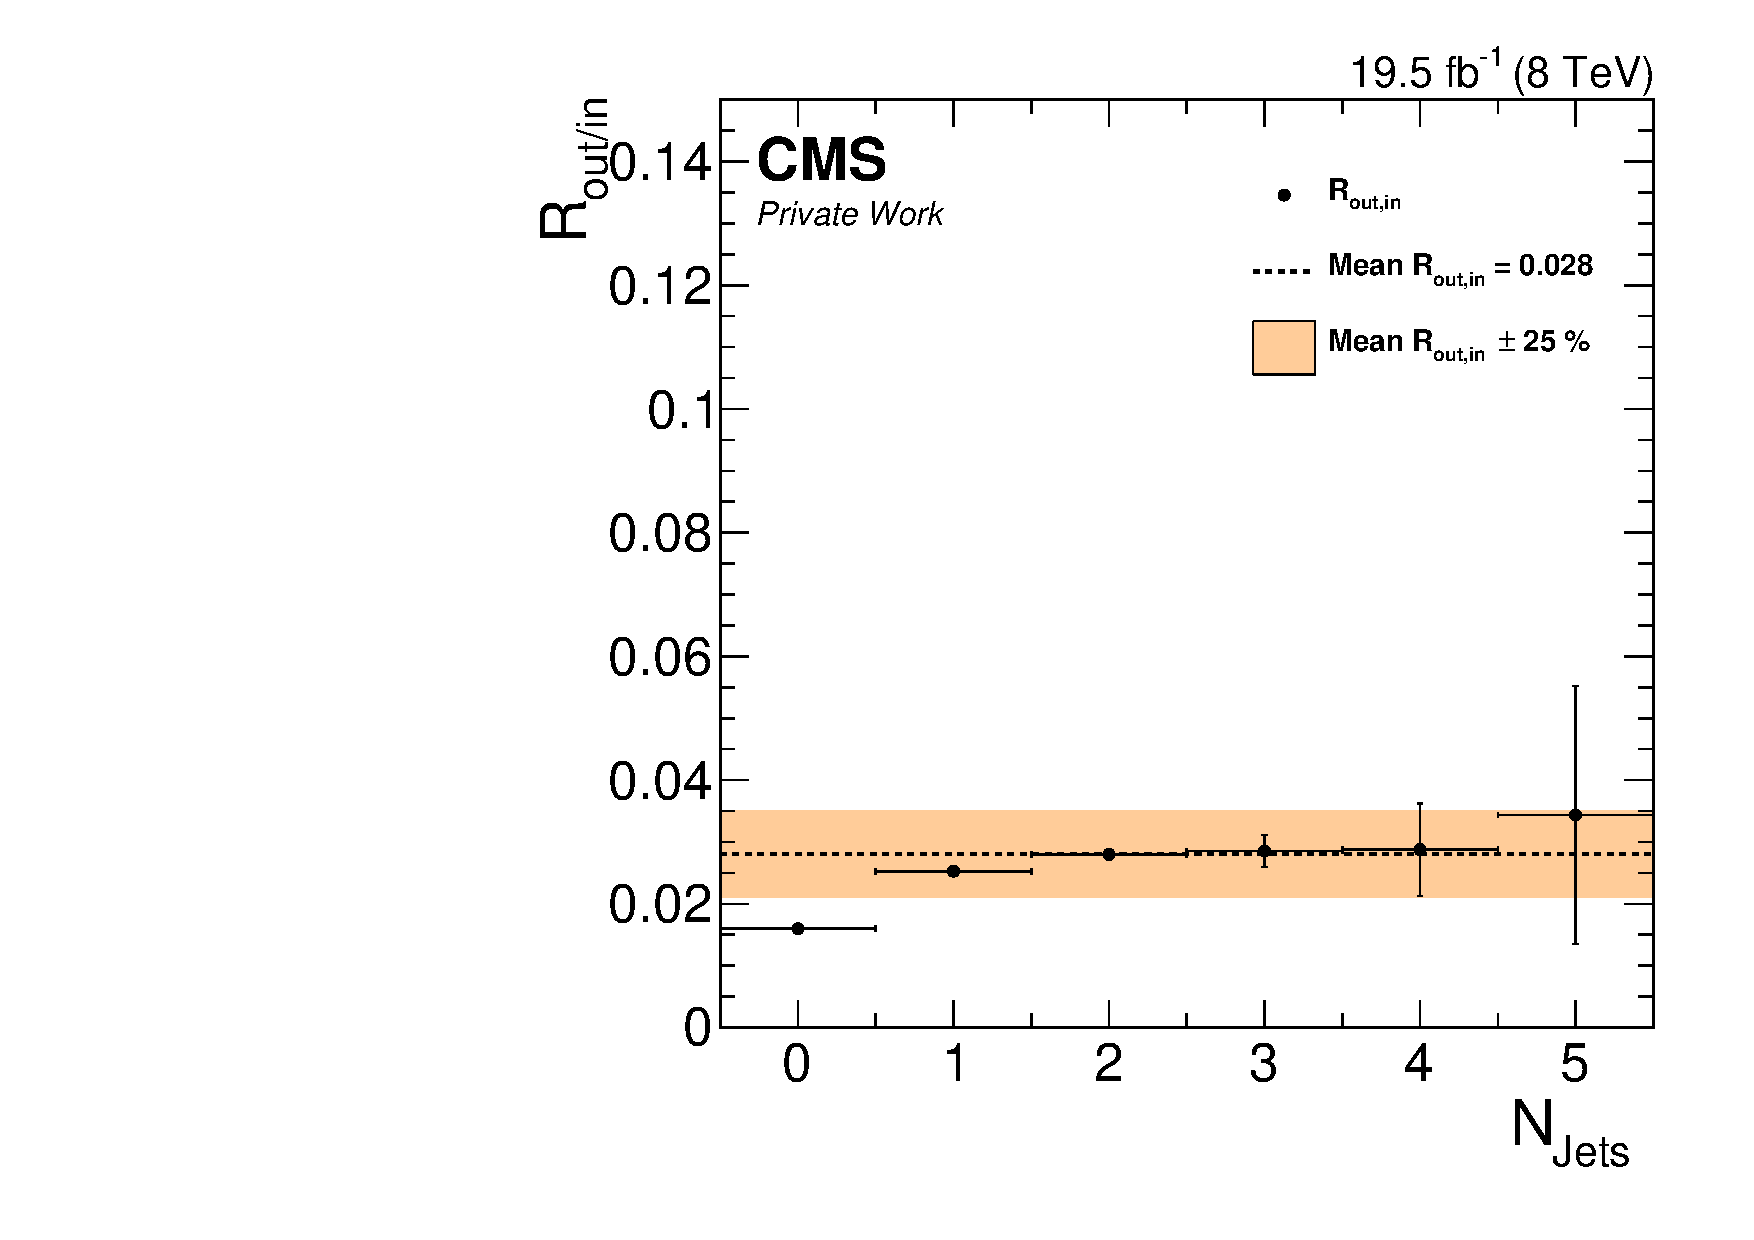
\includegraphics[width=\textwidth]{plots/BG/rOutIn/rOutInSyst_DrellYanControlForward_Full2012_NJets_HighMass_SF_None.pdf}
\end{minipage}
\caption{Dependencies of \Routin for the high-mass region on \MET (left) and \njets (right) for the central (top) and forward (bottom) lepton selection. The results on data are shown in black. The central value is shown as a black dashed line while the systematic uncertainty is shown as an orange band.}
\label{fig:ROutInDependencies2}
\end{figure} 